\subsubsection{Model \textit{Use case}}
\label{subsec:model-usecase}
Dari beberapa kebutuhan fungsional serta karakteristik pengguna, dapat dibuat \textit{use case} yang mengelompokkan serta menggambarkan relasi antara aktor dan aksi yang dapat dilakukan. \textit{Use case} memiliki identifikasi yang berawalan dengan UC diikuti oleh dua angka. \textit{Use case} dapat dilihat secara detail pada lampiran \ref{tab:penjelasan-usecase-diagram}.

Dari pemetaan \textit{use case} pada lampiran \ref{tab:penjelasan-usecase-diagram}, dapat dibuat sebuah diagram yang menghubungkan relasi antara aktor dengan \textit{use case}-nya. Relasi  aktor dengan kapabilitas fungsional sistem dapat dilihat pada diagram use case di Gambar \ref{fig:usecase-diagram}.

\begin{figure}[ht]
  \centering
  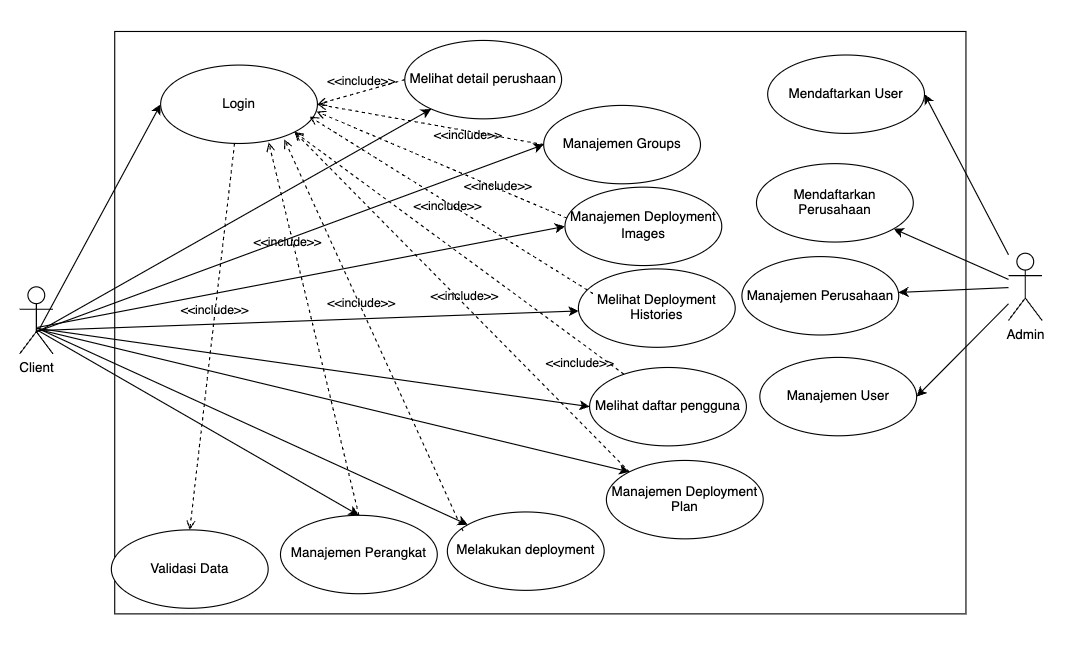
\includegraphics[width=1\textwidth]{resources/chapter-3/usecase-diagram.jpg}
  \caption{Usecase Diagram}
  \label{fig:usecase-diagram}
\end{figure}

\pagebreak